% !TeX root=../main.tex
\chapter{پیاده‌سازی}

% ------------ Section 4.1
\section{نوشتن کد قرارداد}
در این بخش به بررسی مراحل و نحوه نوشتن کد قراردادهوشمند پرداخته می‌شود.

% ------------ Sub Section 4.1.1
\subsection{نیازمندی‌های قراردادهوشمند}
نیازمندی‌های اصلی کاپو به ترتیب زیر است.
\begin{itemize}
  \item
هر آدرس در شبکه بتواند یک داده‌ی متنی را به آسان‌ترین و کم هزینه‌ترین روش ممکن به یک توکن NFT تبدیل کند.
  \item
هر آدرس بتواند توکن‌های خود را به اشخاص دیگر انتقال دهد یا در بازارهای معاملات NFT بفروشد.
  \item
در صفحه اول وبسایت تعداد کل توکن‌های ساخته شده تا به حال و تعداد کل دارندگان توکن نمایش داده شود.
  \item
قابلیت‌های قراردادهوشمند تست شده باشد.
\end{itemize}

% ------------ Sub Section 4.1.2
\section{ارث‌بری}
با توجه به مزایای ذکر شده در مورد استانداردسازی قراردادهای هوشمند، انتخاب درستی است که برای پیاده‌سازی این کاربری از یکی از استانداردها استفاده شود. ارثبری از استانداردهای یک کتابخانه متن‌باز مزایای زیر را فراهم می‌کند.
\begin{itemize}
  \item
به دلیل وجود کدهای پایه به صورت آماده سرعت توسعه پروژه افزایش می‌یابد.
  \item
ارتباط دیگر پروژه‌ها با پروژه کاپو به راحتی انجام می‌شود.
  \item
امینت قرارداد و درستی آن حداقل در سطوح پایه‌ای تا حد خوبی تضمین شده است.
\end{itemize}

قراردادهوشمند کاپو از استاندارد ERC721 پیاده‌سازی شده در کتابخانه اپن‌زپلین
\LTRfootnote{
  \url{https://github.com/OpenZeppelin/openzeppelin-contracts}
}
ارث‌بری میکند که یکی از معروف ترین کتابخانه‌های پیاده کننده استانداردهای قرارداد هوشمند است.

% ------------ Sub Section 4.1.3
\subsection{توجه به هزینه تراکنش و نوع توابع}
در نوشتن یک قراردادهوشمند باید به نکات زیر توجه کنیم.
\begin{itemize}
  \item
میزان حافظه‌ای که اشغال می‌کنیم.
  \item
حجم بایت‌کد.
  \item
میزان عملیات هر متد، به خصوص متدهایی که مکررا مورد استفاده کاربر قرار می‌گیرند.
  \item
نوع هر متد، که مشخص می‌کند هر متد تا چه حد روی شبکه بلاکچین تغییر ایجاد می‌کند.
\end{itemize}

توجه نکردن به هریک از این موضوعات باعث می‌شود که قراردادهوشمند به اندازه کافی بهینه عمل نکند و کاربر وادار به پرداخت gasfee یا هزینه تراکنش بیشتر شود. یکی از مهمترین نکاتی که برای بهینه‌تر رفتار کردن قراردادهوشمند باید به آن توجه کنیم نوع هر متد است.

اگر متدی از نوع pure تعریف شود به این معنی است که به هیچ اطلاعاتی از شبکه بلاک‌چین نیاز ندارد و همه‌ی اطلاعاتی که لازم دارد را در اسکوپ
\LTRfootnote{Scope}
خودش دارد. اگر متدی از نوع view باشد به این معنی است که به اطلاعاتش روی شبکه بلاکچین نیاز دارد اما فقط می‌خواهد که آن‌ها را بخواند و نمیخواهد تغییری در آن‌ها ایجاد کند. این دو نوع متد نیازی به پرداخت کارمزد تراکنش توسط کاربر ندارند، اما اگر در تعریف متدی ذکر نشود که یکی از این دو نوع است، اینطور در نظر گرفته می‌شود که نیاز به بروزرسانی اطلاعاتش در شبکه بلاکچین دارد و از کاربری که آن را فراخوانی کرده است هزینه تراکنش دریافت می‌شود.


% ------------ Sub Section 4.1.4
\subsection{جزئیات فنی پیاده‌سازی}
مینت کردن در این قرارداد به آدرس‌های مشخص محدود نیست و همه می‌توانند توکن بسازند. بسیاری از قراردادها برای صرفه‌جویی در هزینه تراکنش کاربران اکثر اطلاعات مربوط به توکن‌ها را در قرارداد نگه نمیدارند و فقط داده‌های بسیار مهم توکن را در شبکه بلاکچین نگهداری می کنند. از آنجایی که کاپو یک قرارداد همه منظوره است و ممکن است استفاده‌های فراوانی داشته باشد، تصمیم‌گیری این مورد به عهده کاربر قرارداد گذاشته می‌شود.

در کاپو آیدی هر توکن از hash داده‌های توکن به دست می‌آید. این نحوه عملکرد چند مذیت ایجاد می‌کند. به این ترتیب هیچ دو توکنی نمی‌توانند داده‌های یکسان داشته باشند، زیرا در این صورت آیدی آن‌ها باید یکسان باشد و این امکان پذیر نیست زیرا آیدی توکن‌ها یکتاست. همچنین آیدی توکن‌ها دیگر ترتیبی نخواهند بود و ترتیب ساخت توکن‌ها مشخص نخواهد بود.

در یک قرارداد ERC721 استاندارد فقط آیدی توکن‌ها ذخیره می‌شود. در کاپو علاوه بر آیدی توکن‌ها یک map از آیدی توکن‌ها به داده‌ی آن‌ها با نام tokenDatas نیز نگهداری می‌شود. همچنین در کاپو map دیگری نیز از آدرس به لیست توکن‌های آن آدرس با نام ownerTokens نگهداری می‌شود. متغیر اول کمک می‌کند که با داشتن آیدی یک توکن به راحتی داده‌های آن توکن به دست آورده شوند. متغیر دوم نیز کمک می‌کند که به راحتی بتوان توکن‌های یک آدرس را به دست آورد. دومتغیر دیگر با نام‌های numberOfTokenHolders و numberOfMintedTokens نیز در کاپو نگه‌داشته می‌شوند که برای نمایش آمار استفاده از قرارداد در صفحه اصلی اپلیکیشن مورد استفاده قرار می‌گیرند.

متد mint به نحوی نوشته شده است که برای عموم قابل استفاده باشد. پس از محاسبه hash داده‌ی توکن از آن به عنوان آیدی توکن استفاده میکند، توکن را می‌سازد و متغیرهای tokenDatas و numberOfMintedTokens را بروزرسانی می‌کند.

\begin{figure}[ht]
\centerline{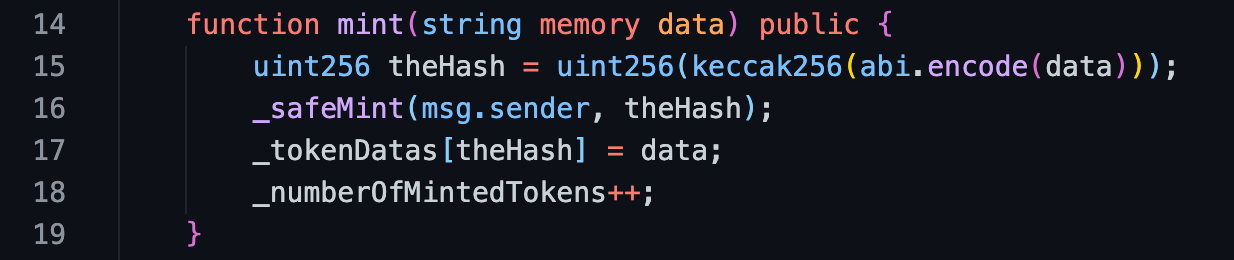
\includegraphics[width=12cm]{mint.png}}
\caption{پیاده‌سازی تابع mint}
\label{fig:mint}
\end{figure}

متد afterTokenTransfer از استاندارد ERC721 به نحوی بازنویسی
\LTRfootnote{Overwrite}
شده است که پس از هر انتقال توکن با بررسی آدرس‌های مبدا و مقصد، متغیر‌های numberOfTokenHolders و numberOfMintedTokens و ownerTokens را بروزرسانی کند.

\begin{figure}[ht]
\centerline{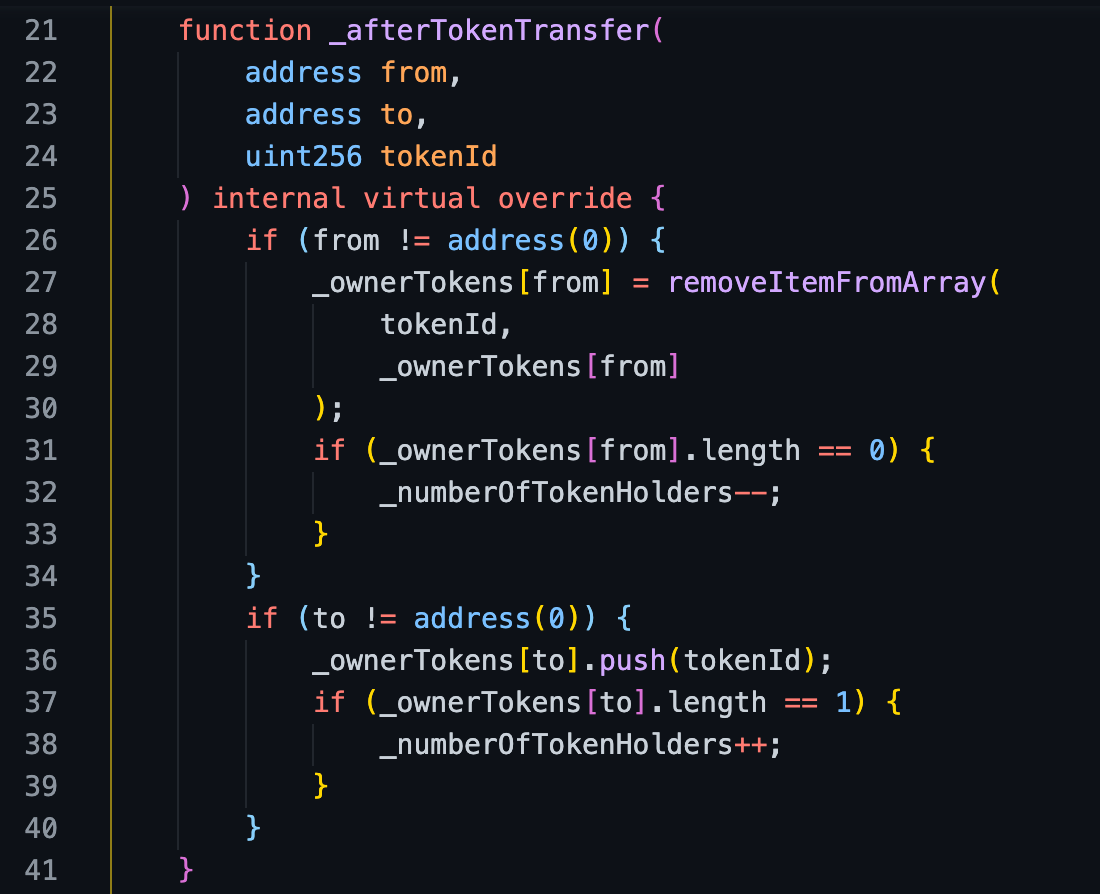
\includegraphics[width=12cm]{afterTokenTransfer.png}}
\caption{پیاده‌سازی تابع afterTokenTransfer}
\label{fig:afterTokenTransfer}
\end{figure}

متد جدیدی با نام getUserTokens نیز نوشته شده است که در استاندارد ERC721 به صورت پیش‌فرض وجود ندارد. این متد با گرفتن یک آدرس و استفاده از ownerTokens و tokenDatas دو خروجی برمی‌گرداند، لیستی از آیدی توکن‌های آدرس و لیستی از داده‌های توکن‌های آدرس.

\begin{figure}[ht]
\centerline{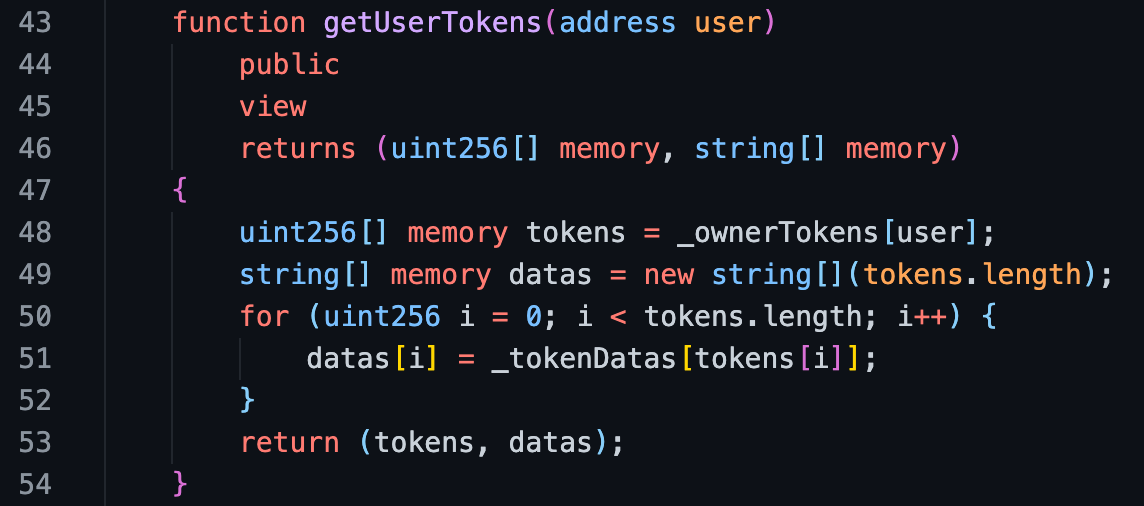
\includegraphics[width=12cm]{getUserTokens.png}}
\caption{پیاده‌سازی تابع getUserTokens}
\label{fig:getUserTokens}
\end{figure}

همچنین از آنجایی که سالیدیتی به طور پیش‌فرض امکان حذف یک داده از یک آرایه با داشتن مقدار آن را ندارد، عدم وجود این قابلیت هزینه‌بر بودن آن است، در سالیدیتی توسعه دهندگان به استفاده از map و دوری از array ها تشویق می‌شوند. اما برای نمایش نحوه ارث‌بری از دو یا چند قرارداد پدر، برای کاپو یک قرارداد به نام Helper نوشته شد که این قابلیت را فراهم می‌کند. کاپو علاوه بر
\lr{ERC721}
از قرارداد Helper نیز ارث‌بری می‌کند.

\begin{figure}[ht]
\centerline{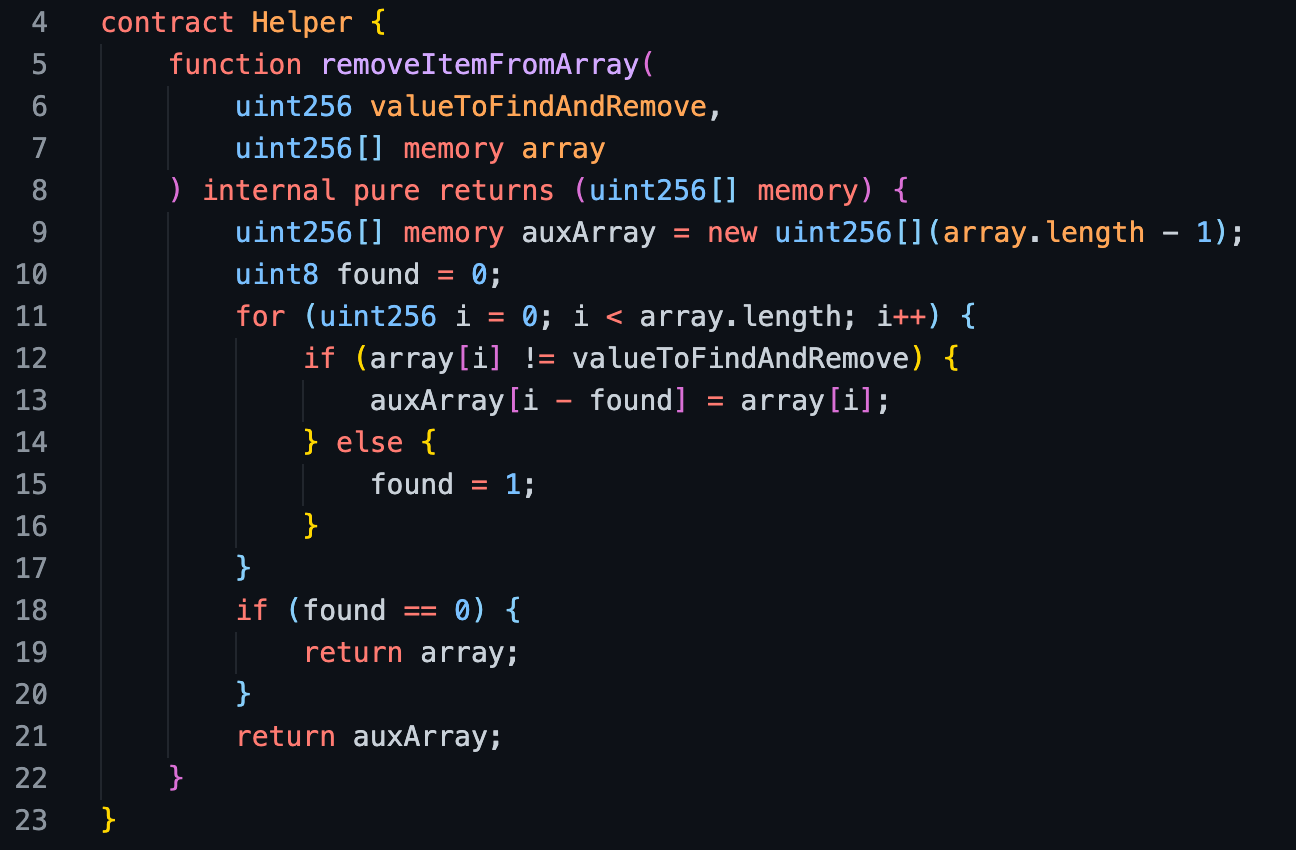
\includegraphics[width=12cm]{Helper.png}}
\caption{پیاده‌سازی قرارداد Helper}
\label{fig:Helper}
\end{figure}

% ------------ Section 4.2
